\documentclass[10pt,pdf,hyperref={unicode}]{beamer}

\mode<presentation>
{
\usetheme{boxes}
\beamertemplatenavigationsymbolsempty

\setbeamertemplate{footline}[page number]
\setbeamersize{text margin left=0.5em, text margin right=0.5em}
}

\usepackage[utf8]{inputenc}
\usepackage[main=russian, english]{babel}
\usepackage{bm}
\usepackage{multirow}
\usepackage{ragged2e}
\usepackage{indentfirst}
\usepackage{multicol}
\usepackage{subfig}
\usepackage{amsmath,amssymb}
\usepackage{enumerate}
\usepackage{mathtools}
\usepackage{comment}
\usepackage{multicol}
\usepackage{hyperref}

\usepackage[all]{xy}

\usepackage{tikz}
\usetikzlibrary{positioning,arrows}

\tikzstyle{name} = [parameters]
\definecolor{name}{rgb}{0.5,0.5,0.5}

\usepackage{caption}
\captionsetup{skip=0pt,belowskip=0pt}

\newtheorem{rustheorem}{Теорема}
\newtheorem{russtatement}{Утверждение}
\newtheorem{rusdefinition}{Определение}

% colors
\definecolor{darkgreen}{rgb}{0.0, 0.2, 0.13}
\definecolor{darkcyan}{rgb}{0.0, 0.55, 0.55}

\AtBeginEnvironment{figure}{\setcounter{subfigure}{0}}

\captionsetup[subfloat]{labelformat=empty}

%----------------------------------------------------------------------------------------------------------

\title[]{Состязательные Мосты Шрёдингера}
\author{Ксенофонтов\,Г.\,С.\\[1ex] 
\small Научный руководитель: Исаченко\,Р.\,В.,\ к.ф.-м.н.}
\institute[]{Московский физико-технический институт (национальный исследовательский университет)}
\date[2023]{\small 18\;мая\;2024}

%---------------------------------------------------------------------------------------------------------
\begin{document}

\begin{frame}
\titlepage
\end{frame}

%---------------------------------------------------------------------------------------------------------- This implies that a learner has only a sample access to the (continuous) distributions and based on it has to recover the entire SB process (e.g., its drift) between the entire distributions.
\section{Исследование}
\begin{frame}{Задача мостов Шрёдингера}
    \bigskip
    \begin{block}{Цель}
        Найти прямое и обратное отображения между двумя распределениями данных с использованием мостов Шрёдингера.
    \end{block}
    \begin{block}{Задача}
        \justifying
        Разработать метод нахождения отображений, который не строит стохастического процесса между распределениями, и который не страдает от проклятия размерности.
    \end{block}
    \begin{block}{Решение}
        Использовать эквивалентную задачу мостов Шрёдингера совместно с состязательное обучением.
    \end{block}
\end{frame}
% %---------------------------------------------------------------------------------------------------------

\section{Постановка проблемы}
\begin{frame}{Постановка проблемы}
Пусть дано:
\begin{enumerate}[1.]
    \item $\{x_i\}_{i=0}^N = X, \{y_j\}_{j=0}^M = Y$ -- два непарных набора данных,  где $x \sim \pi_0(x)$ и $y \sim \pi_T(y)$,
    \item $p^{\mathbb{W}^{\gamma}}(x_0, \dots, x_T)$ -- совместное распределение эталонного Винеровского процесса с коэффициентом смещения $\sqrt{\gamma}$, а $x_0$ и $x_T$ -- элементы из $X$ и $Y$, соответственно.
\end{enumerate}

Динамическая постановка мостов Шредингера:

\begin{equation}
    q^*(x_0, \dots, x_T) = \arg\min_{q\in \mathcal{D}(\pi_0, \pi_T)} D_{KL}(q(x_0, \dots, x_T)||p^{\mathbb{W}^{\gamma}}(x_0, \dots, x_T)),
    \label{eq:dyn}
\end{equation}

где $\mathcal{D}(\pi_0, \pi_T)$ множество всех совместных маргинальными распределениями $\pi_0(x_0)$ и $\pi_T(x_T)$.

\begin{alertblock}{Проблема}
    Для моделирования процесса используется сложная марковская цепь, которая значительно усложняет процесс генерации/инференса.
    \begin{equation*}
        q(\textcolor{red}{x_0, \dots, x_T}) = \pi_1(x_T) \prod_{t=0}^{T-1} q_{t|t+1} (x_t | x_{t+1}),
    \end{equation*}
\end{alertblock}
\end{frame}

% %----------------------------------------------------------------------------------------------------------
\section{Предложенный метод}
\begin{frame}{Предложенное решение}
~\\[-1mm]
\begin{block}{Статическая постановка задачи мостов Шрёдингера}
    \begin{equation}
        q^*(x,y) = \arg\min_{q\in \mathcal{D}(\pi_0, \pi_T)} D_{KL}(q(x,y)||p^{\mathbb{W}^\gamma}(x,y)),
        \label{eq:static}
    \end{equation}
\end{block}


Такая задача решается с помощью итеративного алгоритма Iterational Proportional Fitting (IPF):
\begin{equation*}
    \begin{split}
        \color{blue}p^*(x,y) = \arg\min_{p\in \mathcal{D}(\cdot, \pi_T)}D_{KL}(p(x,y)||q^*(x,y)), \\
        \color{violet}q^*(x,y) = \arg\min_{q\in \mathcal{D}(\pi_0, \cdot)}D_{KL}(q(x,y)||p^*(x,y))
    \end{split}
\end{equation*}

Продемонстрируем предложенный метод на примере \textcolor{blue}{обратного} шага:
\begin{equation*}
    p^*(x,y) = \arg\min_{p\in\mathcal{D}(\cdot, \pi_T)}\max_{D}\mathbb{E}_{(x,y)\sim p}\left[D(x,y)\right] - \mathbb{E}_{(x,y)\sim q^*}\left[e^{D(x,y) - 1}\right]
\end{equation*}

\footnotetext[1]{\href{https://arxiv.org/abs/1606.00709}{f-GAN: Training Generative Neural Samplers using Variational Divergence Minimization}}
\end{frame}

\begin{frame}{Иллюстрация IPF}
~\\[-1mm]
    \begin{figure}
        \centering
        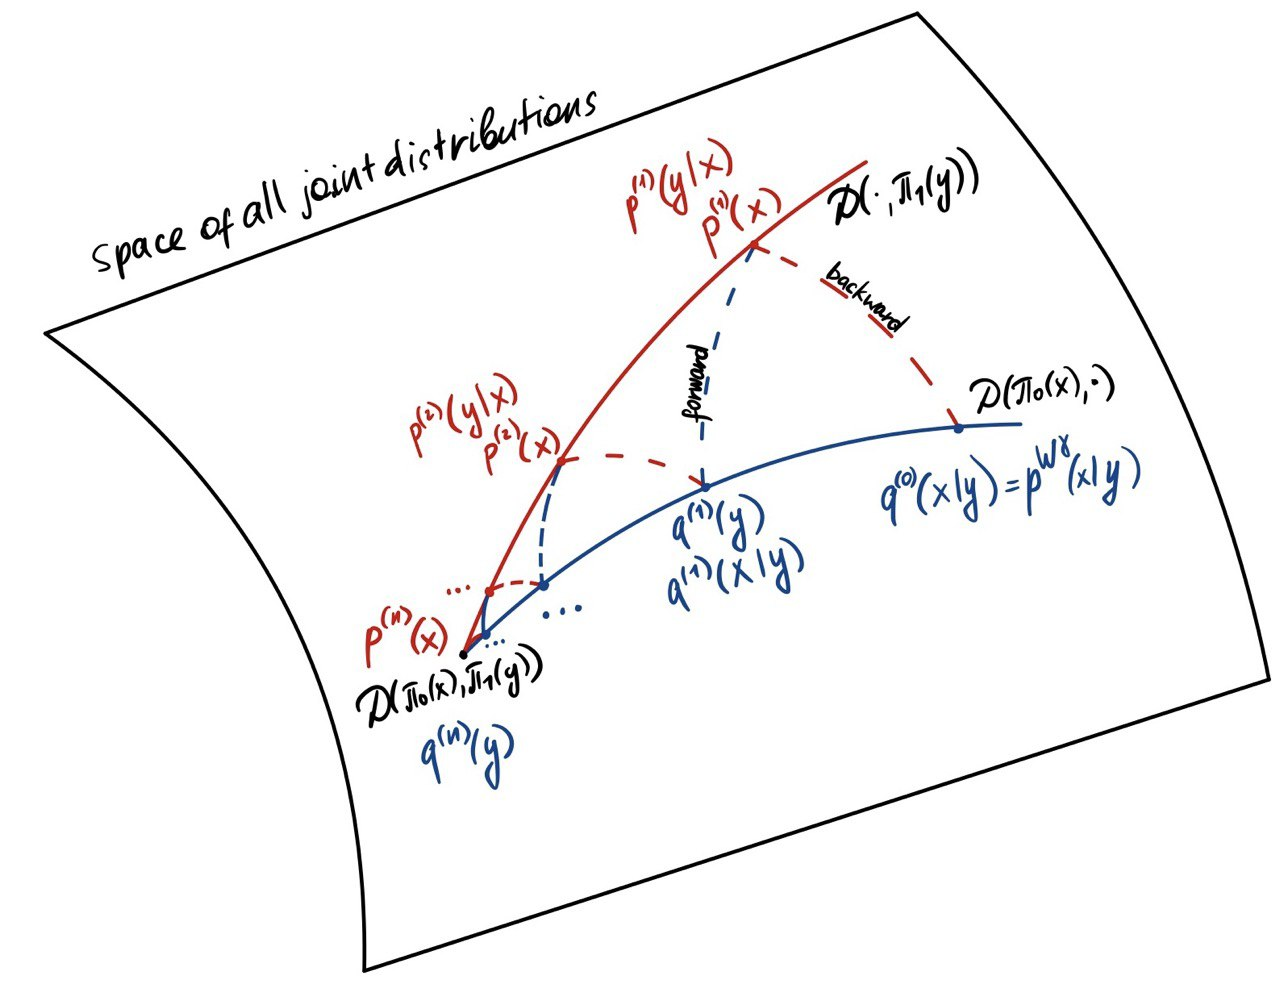
\includegraphics[width=0.8\linewidth]{slides/3d/figures/photo_2023-12-16_13-49-39.jpg}
    \end{figure}
\end{frame}

\begin{frame}{Предложенный метод}
    ~\\[-1mm]
    Разложим мат. ожидания и введем генератор\footnote{\href{https://arxiv.org/abs/1411.1784}{Conditional Generative Adversarial Nets}}:
    \begin{equation*}
        \begin{split}
             \min_{\textcolor{red}{p(x,y)\in\mathcal{D}(\cdot, \pi_T)}}\max_{D}\textcolor{blue}{\mathbb{E}_{(x,y)\sim p(x,y)}}\left[D(x,y)\right] - \textcolor{violet}{\mathbb{E}_{(x,y)\sim q^*(x,y)}}\left[e^{D(x,y) - 1}\right] = \\ = \min_{\textcolor{red}{p(x|y)}}\max_{D}\textcolor{blue}{\mathbb{E}_{y \sim \pi_T}\mathbb{E}_{x\sim p(x|y)}}\left[D(x,y)\right] - \textcolor{violet}{\mathbb{E}_{x\sim\pi_0}\mathbb{E}_{y\sim q^*(y|x)}}\left[e^{D(x,y) - 1}\right] = \\ = \min_{\textcolor{red}{G}}\max_{D}\mathbb{E}_{y \sim \pi_T}\textcolor{blue}{\mathbb{E}_{z\sim p(z)}}\left[D\left(G(z,y),y\right)\right] - \mathbb{E}_{x\sim\pi_0}\textcolor{violet}{\mathbb{E}_{z\sim p(z)}}\left[e^{D(x,F^*(z,x)) - 1}\right],
        \end{split}
    \end{equation*}
    где $G$, $F$, $D$ - генераторы и дискриминатор, параметризованные нейронными сетями.
\end{frame}



%----------------------------------------------------------------------------------------------------------
\section{Эксперименты}
\begin{frame}{Демонстарция метода на игрушечном 2D наборе данных }
    \justifying
    \begin{figure}
        \centering
        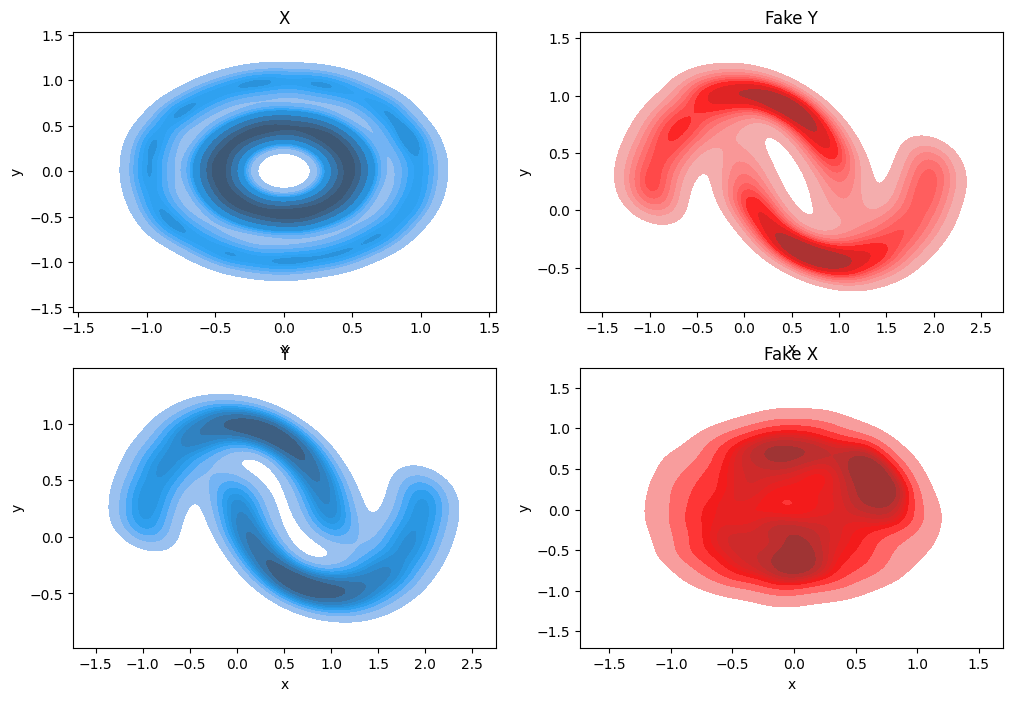
\includegraphics[width=0.7\linewidth]{slides//4th//figures/2d_toy.png}
    \end{figure}
\end{frame}

\begin{frame}{Коллапс моды}
    \justifying
    Как и все GAN модели, данный подход очень чувствителен к подбору гиперпараметров. Неаккуратный выбор может привести к коллапсу моды.
    \begin{figure}
        \centering
        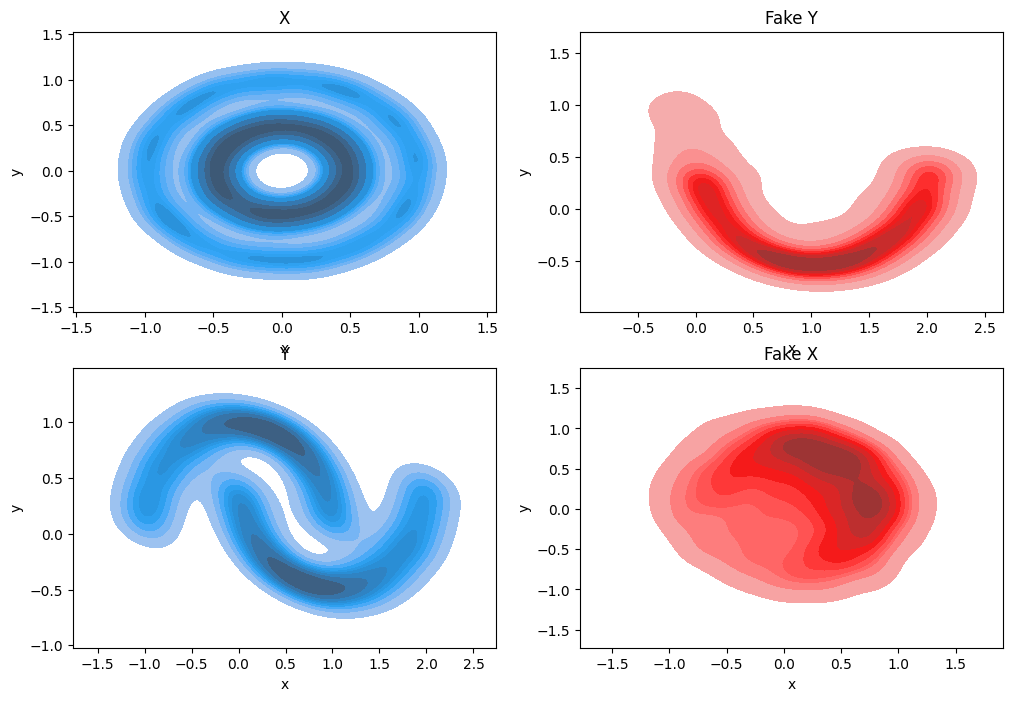
\includegraphics[width=0.8\linewidth]{slides//4th//figures/mode_collapse.png}
    \end{figure}
\end{frame}


%----------------------------------------------------------------------------------------------------------
\section{Вывод}
\begin{frame}{Выносится на защиту}
\justifying
    \begin{enumerate}
        \justifying
        \item Предложен метод, который не строит стохастического процесса между распределениями, и который не страдает от проклятия размерности.
        \item Проведены эксперименты и выявлены недостатки подхода. 
    \end{enumerate}
\end{frame}

\end{document} 